\begin{problem}{Защита лилипутов}{стандартный ввод}{стандартный вывод}{1 секунда}{256 мегабайт}

Населению Лилипутии с давних пор угрожают титаны-лилипутоеды. Для защиты от них лилипуты возводят большие стены, имеющие вид окружностей, некоторые из которых могут размещаться внутри других. Уже практически целый век лилипуты живут спокойно и даже начали забывать о беспощадных врагах. Но с приходом Колоссальных титанов, способных разрушать стены, лилипутское общество вновь оказалось в опасности.

Известно, что в Лилипутии есть $n$ стен, и любые две стены либо не пересекаются, либо вложены друг в друга. Колоссальных титанов оказалось так много, что в некоторый момент времени они могут сломать все внешние стены одновременно, и тогда лилипуты будут вынуждены отступить под защиту более внутренних стен. 

Время на исходе, лилипуты паникуют. Король лилипутов обратился к вам за помощью, чтобы решить, куда лучше всего бежать. Помогите ему найти стену, которая падет последней. 



\InputFile
В первой строке задано натуральное число $n$ $(1 \leq n \leq 2 \cdot 10^3)$. 

В оставшихся $n$ строках содержатся описания стен-окружностей~--- координаты центра $(x_{i}, y_{i})$ и радиус $r_{i}$ $(1 \leq r_{i}, x_{i}, y_{i} \leq 10^8, 0\leq x_{i} - r, y_{i} - r \leq 10^8)$ каждой $i$-й окружности $(i = 1, \dots, n)$.

\OutputFile
Выведите порядковый номер самой внутренней стены (нумерация стен начинается с 1). Если ответов несколько, выведите любой из них.

\Examples

\begin{example}
\exmpfile{example.01}{example.01.a}%
\exmpfile{example.02}{example.02.a}%
\end{example}

\Note
\begin{center}
  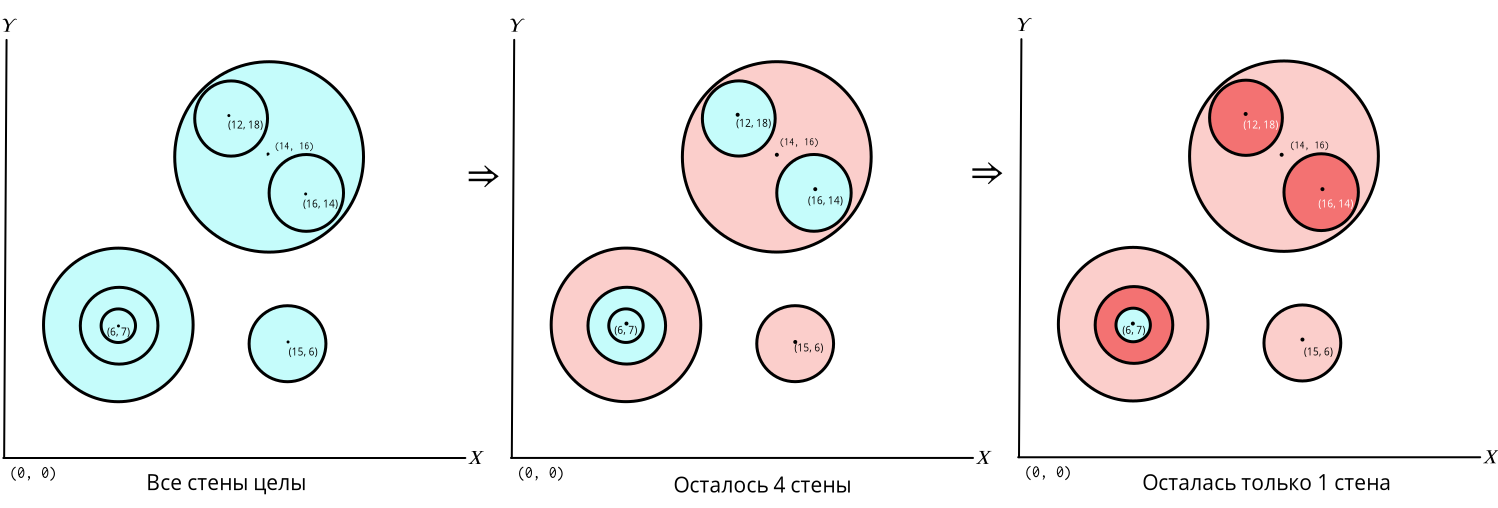
\includegraphics[width=18cm]{sample2.png}
\end{center}
На рисунках изменением цвета показано, в каком порядке как будут рушиться стены во втором примере. Последней падет стена под номером 4 с радиусом 5 и центром $(6, 7)$.

\end{problem}

